\section{Query}

Im folgenden führen wir in den von Redmond et al. verwendeten Query-Begriff ein.
Hierbei betrachten wir dessen Notation als auch Auswertung.\\
Zunächst motivieren wir die idiomatische ECS-Datenstruktur unter Anwendung des Funktionalen Abhängigkeits-Begriffs, um auf dieser Grundlage im späteren Verlauf einige Operationen exemplarisch darzustellen.\\

\subsection*{Relationales Schema des ECS}
Ein erster Entwurf eines relationalen Schemas der bislang behandelten zentralen Begriffe \textit{Entitäten} und \textit{Komponenten} führt zu dem in Abbildung~\ref{fig:relation} dargestellten Schema, der den Entitätstyp $E$ als auch zwei  Komponententypen $K_i$, $K_j$ enthält.\\
Hierbei wird der  Entitätstyp $E$ mit den Komponententypen in binäre Relationen überführt -- die Darstellung entspricht damit einer in vorherigen Abschnitten bereits erwähnten \textit{entitätszentrischen} Darstellung und wird schematisch in ähnlicher Form genutzt~\cite[Fig.1, 272:3]{RCCM+25}.


\begin{figure}[!htbp]
    \centering
    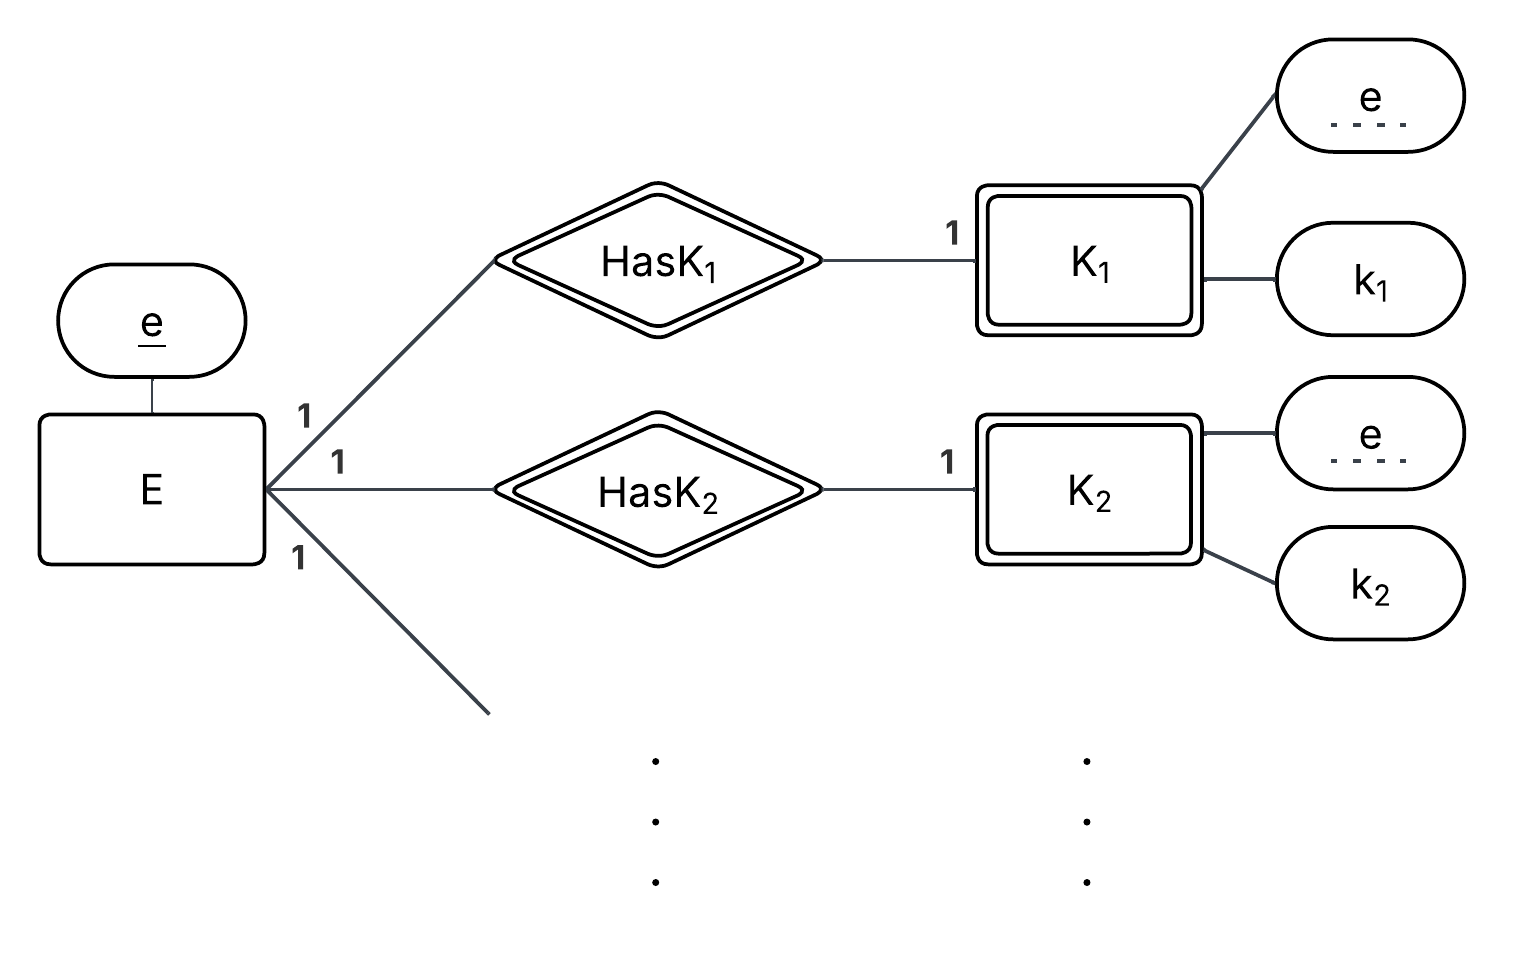
\includegraphics[width=0.6\columnwidth]{content/de/appendix/concurrency_paper/notation/img/relation}
    \caption{ER-Modell von Entität und Komponenten als entitätszentrischer Entwurf. Bei der Notation folgen wir Chen~\cite{Che76}. (Quelle: eigene Darstellung)}
    \label{fig:relation}
\end{figure}

In den folgenden Schritten überführen wir den Entwurf in die ECS-idiomatische komponentenzentrische Darstellung, wobei wir uns bei Begriffen und Vorgehen an Elmasri und Navathe orientieren~\cite{EN11}.\\

Relation und Attributmengen sind hierbei wie folgt gegeben:

\[
    \begin{alignat}{3}
     E &= \{e\}\\
     K_i &= \{e, k_i\}\\
     K_i &= \{e, k_j\}\\
    \end{alignat}
\]

\noindent
Wir identifizieren den Primärschlüssels $e$, der in der Relation $E$ eine triviale funktionale Abhängigkeit $e \rightarrow e$ aufweist, sowie in den anderen Relationen jeweils $e \rightarrow k_i$ bzw. $e \rightarrow k_j$.\\

\noindent
Die funktionale Abhängigkeitsmenge $F$ lautet damit entsprechend

\[
    \begin{alignat}{3}
    F = &\{\\
        &e \rightarrow \{k_i, k_j\}\\
    & \}\\
    \end{alignat}\ ,
\]

\noindent
woraus sich die Hülle von $e$ unter $F$ ableiten lässt:

\[
    e^+ =\{e, k_i, k_j\}
\]

\noindent
Damit können wir die Menge der minimalen funktionalen Abhängigkeitsmenge $F_\text{min}$ bestimmen, um redundante Informationen zu entfernen:
\[
    \begin{alignat}{3}
    F_\text{min} = &\{
        &e \rightarrow {k_i},
        &e \rightarrow {k_j}
    &\}
    \end{alignat}
\]

\noindent
Die resultierenden funktionalen Abhängigkeiten können in ein Relationschema

\[
    K\ (e,\ k_i,\ k_j)
\]

\noindent
überführt werden, die nicht weiter normalisiert werden braucht.
Es ist sofort klar, dass eine solches Schema möglicherweise NULL-Werte für $k_i$ oder $k_i$ enthalten wird.\footnote{
    Codd diskutiert die Auswirkungen von NULL-Werten -- auch im Hinblick auf Normalisierung -- in~\cite{Cod86}; weitere Betrachtung und formalen und semantischen Aspekten bei Franconi und Tessaris~\cite{FT22}.
}\\
Damit würde für jedes $k_i$, das für $e \in E$ erstellt wird, auch ein $k_j$ erstellt werden und umgekehrt.
Für das formale Modell spielt dies keine Rolle - hätte aber in einer entsprechenden Anwendungsnahen Implementierung den Effekt, dass nicht auf Vorhandensein einer Assooziation $e \mapsto k_j$ geprüft werden muss, sondern der enthaltene Wert.
Außerdem trägt ein Schema zwei domänenspezifische Typen, was die Semantik des Datenmodells abschwächt.
\\

Aus diesem Grund dekomponieren wir die Relation und erhalten das Relationsschema wie in Abbildung~\ref{fig:relation_ecs}
dargestellt.\footnote{
Eine formale Grundlage für diese Form liefert die 6ste Normalform~\cite[S. 176]{DDL03}
}

\[
    \begin{alignat}{3}
    K_i(e,\ k_i)\\
    K_j(e,\ k_j)\\
    \end{alignat}
\]


\begin{figure}[!htbp]
    \centering
    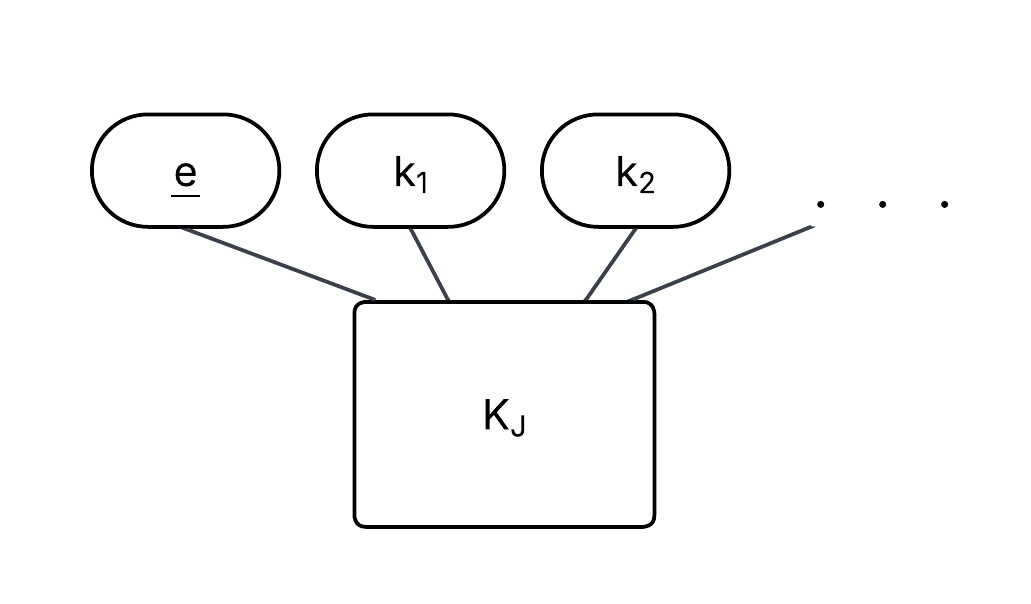
\includegraphics[width=0.6\columnwidth]{content/de/appendix/concurrency_paper/notation/img/relation_ecs}
    \caption{Nach bestimmung der funktionalen Abhängigkeiten können wir mit hilfe der minimalen funktionalen Abhängigkeitsmenge auf ein normalisiertes Schema zuückgreifen, dass die komponentenzentrische, idiomatische Datenverwaltung in einem ECS repräsentiert..  (Quelle: eigene Darstellung)}
    \label{fig:relation_ecs}
\end{figure}



\subsection*{Semantik und Auswertung von Queries}

Im Zusammenhang mit Queries führen die Autoren folgende Notationen ein:\footnote{
 Sogenannte ``Denotation Brackets``~\cite{Rab17}.
}

\[
    \llbracket - \rrbracket_c
\]
\bigskip

Dabei ist $\llbracket\ - \rrbracket_c$ eine Funktion, die im Zustand $c$ des \textit{Core ECS}-Programms als Parameter eine Query beziehungsweise einen Query-Constraint erhält und dabei eine oder mehrere partielle Abbildungen zurückgibt, die die Query-Bedingungen erfüllen.
Dabei enthält der Definitionsbereich stets eine Teilmenge von Entitätsterme vom Typ \ty{E}; der Wertebereich wird über die Query-Bedingung vorgegeben:

\bisgskip
\[
    \begin{alignedat}{3}
        \llbracket\ \tm{incl}_i\ \rrbracket_c &\coloneqq c_i
        \\[1mm]
        \llbracket\ \tm{excl}_i\ \rrbracket_c &\coloneqq \{*\}_{\ty{e} \in \text{live}(c)\backslash\text{dom}(c_i)}
        \\[1mm]
        \llbracket\ \tm{anyway}_i\ \rrbracket_c &\coloneqq c_i\  \dot\cup\ \{*\}_{\ty{e} \in \text{live}(c)\backslash\text{dom}(c_i)}
        \\[1mm]
        \llbracket\ \nt{q} \land \nt{q'}\ \rrbracket_c &\coloneqq \{ (\ \llbracket \nt{q} \rrbracket_c(\ty{e}),\ \llbracket \nt{q'} \rrbracket_c(\ty{e})\ ) \}_{e \in \text{live}(c)}
        \\[1mm]
    \end{alignedat}
\]
\bigskip

\noindent
Hierbei ist \texttt{*} definiert als \textit{unit}, und hat den Typ $\top$~\cite[S.118--119]{Pie02}.
Er wird genutzt, um partielle Abbildungen zu repräsentieren, die als Ergebnis einer Query keine konkrete Komponentenassoziation repräsentieren, beispielsweise bei \tm{excl}:

\[
    E \rightharpoonup \top, e \mapsto *
\]



\noindent
Die Semantik der Funktionen bezüglich des Zustandes $c$ lässt sich damit wie folgt beschreiben:

\begin{itemize}
    \itemsep0.5em
    \item $\llbracket\ \tm{incl}_i\ \rrbracket_c$: Die Menge der partiellen Abbildungen der Entitätsterme, die eine Assoziation zu dem Komponententyp $K_i$ haben.
    \item $\llbracket\ \tm{excl}_i\ \rrbracket_c $: Die Menge der Abbildungen von Entitätsterme, bei denen $e \in E$ eine Assoziation zu einem beliebigen komponententerm besitzen,  aber keine zu dem Komponententyp $K_i$ besitzen.
    Da diese Abbildungen keinen assoziierten Komponententypen haben, nutzen die Autoren hierzu \texttt{*} vom Typ $\top$.
    \item $\llbracket\ \tm{anyway}_i\ \rrbracket_c$: Die Menge der Abbildungen von Entitätsterme, die entweder eine Assoziation zu dem Komponententyp $K_i$ besitzen, oder nicht.
    In letztem Fall wird wieder \texttt{*} zur Repräsentation der Assoziationen genutzt.
    \item $\llbracket\ \nt{q} \land \nt{q'}\ \rrbracket_c$: Die Menge der Abbildungen von Entitätsterme, bei denen \ty{e} die über \nt{q} als auch \nt{q'} vorgegebenen Einschränkungen erfüllen.
    Die Semantik ist damit an eine existierende, beliebige Komponentenassoziation von \ty{e} gebunden.
\end{itemize}

\noindent
Die Notation

\[
    \llparenthesis - \rrparenthesis
\]


\noindent
wird verwendet, um den Typ der Rückgabe zu notieren.
Zusammen mit der Semantik der einzelnen Queries ergibt sicht damit\footnote{
Redmon et al. verwenden in $\llparenthesis \tm{anyway_i}\ \rrparenthesis  \coloneqq K_i \cup \top$ anstelle des Vereinigungsoperators $\cup$ das Symbol $+$.
}


\[
    \begin{alignat}{3}
    \llparenthesis\ \tm{incl_i}\ \rrparenthesis  &\coloneqq K_i\\
    \llparenthesis\  \tm{excl_i}\ \rrparenthesis  &\coloneqq \top \\
    \llparenthesis\  \tm{anyway_i}\ \rrparenthesis  &\coloneqq K_i \cup \top\\
    \llparenthesis\  \nt{q}\ \tm{\land}\ \nt{q'} \ \rrparenthesis  &\coloneqq \llparenthesis\  \nt{q} \ \rrparenthesis  \times \llparenthesis\  \nt{q'} \ \rrparenthesis 
    \end{alignat}
\]

\bigskip
\noindent
Hierbei is

\[
    \llparenthesis\  \nt{q} \ \rrparenthesis  \times \llparenthesis\  \nt{q'} \ \rrparenthesis 
\]

\noindent
das kartesische Produkt der durch $\tm{q}$ und $\tm{q'}$ bestimmten Ergebnistypen, beispielsweise für $\llparenthesis \ \tm{incl_i} \land \tm{excl_j} \ \rrparenthesis$

\[
    K_i \times \top
\]

\noindent
oder, bei verschachtelten Queries wie  $\llparenthesis \ (\tm{incl_i} \land \tm{excl_j}) \land \tm{incl_k} \ \rrparenthesis $,


\[
     (K_i \times \top) \times  K_k
\]

\subsection*{Relationale Operationen}

Redmond et {al.} charakterisieren das Anfragesystem von \textit{Core ECS} als ein \textit{konjunktives Anfragesystem}~\cite[S.37--63]{AHV95},
das Selektion $\sigma$, Projektion $\pi$ und binäre Joins $\bowtie$ unterstützt.\\

\noindent
Wir geben im Folgenden ergänzend die Notation für die einzelnen Operationen im Kontext eines auf \textit{Core ECS}-basierenden Systems an und stützen uns dabei auf die geläufige Schreibweise, ohne detailliert darauf einzugehen, legen aber in Anlehnung an Elmasri und Navathe~\cite[S. 137--140]{EN11} wie folgt fest:

\begin{itemize}
    \item Ein Relationsschema $R$ wird als Tupelmenge $R(A_1, A_2, \ldots, A_n)$ definiert, wobei $A_1, \ldots A_n$ die Attributnamen der Relation bezeichnen.
    \item Der Relationszustand $r(R)$ ist definiert als $r(R) \subseteq (\text{dom}(A_1) \times \text{dom}(A_2) \times \ldots \times \text{dom}(A_n))$
    \item Das Relationsschema $R_{K_i}$ ist definiert als
    \[
         R_{K_i} \coloneqq R(\mathcal{E}_i, \mathcal{I}), i \in I
    \]
    mit
    \[
        r(R_{K_i}) \subseteq (\text{dom}(c_i) = \text{dom}(\mathcal{E}_i) \times \text{dom}(\mathcal{I}))
    \]
    \item Das Relationsschema $R_\text{live}$ ist definiert als die Vereinigung aller Relationschemas
    \[
        R_\text{live} \coloneqq R^{\mid K \mid}, R(0) = \mathcal{E}, R(n + 1) = R_{K_i}(2), 0 \leq n \leq \mid K \mid
    \]
\end{itemize}

\noindent
Wir definieren hierzu im Folgenden ein Relationsschema $R_{K_i}$, wobei $R$ als Symbol für \textit{Relationsschema} verwendet wird:


\subsubsection*{Selektion}

Redmond et al. nennen \tm{incl_i} und \tm{excl_i} als Selektionsoperatoren.\\

Zur Ermittlung der Tupel $(e_\text{Position}, k_i)$ für die $e_\text{Position} \in \text{dom}(c_\text{Position}), k_i \in K_i$ gilt, kann geschrieben werden:

\[
    \sigma_{\mathcal{E}_\text{Position} \in \text{live}(c) } (R_{K_\text{Position}}) = \{ (e_i, k_i) \mid e_i \in E, k_i \in K_i, i =\text{Position}  \}
\]

\noindent
Entsprechend kann eine Projektion, die nur den Entitätsterm des Anfrageergebnisses liefert, formuliert werden als


\[
    \pi_{\mathcal{E}_\text{Position}} (\ \sigma (R_{K_\text{Position}})\ ) = \{ e_i \mid e_i in E, i =\text{Position}  \}
\]

\bigskip
\noindent
Um $\tm{excl_i}$ als Selektion anzuwenden,
\[
    \sigma_{R_\text{live}.\mathcal{E}_\text{Position}\ \notin \ \text{dom}(c_\text{Position}) } (R_\text{Live}) = \{(e_i, k_i) \mid e_i \in E, k_i \in I, I \neq \text{Position} \}
\]

\begin{example}[Verschachtelte binäre Query]

    Sei eine Query gegeben, die alle Entitäten $e \in E$ ermittelt, die die Komponente \texttt{Position} sowie \texttt{Collider},
    aber nicht \texttt{Velocity} haben.folgende binäre Query gegeben:

    \[

    \]

    \label{ex:bin_query}
\end{example}